\documentclass[10pt,a4paper,oneside]{article}
\usepackage[utf8]{inputenc}
\usepackage{amsmath}
\usepackage{amsfonts}
\usepackage{amssymb}
\usepackage{draftwatermark} % 设置水印
\SetWatermarkText{DNV Group} % 水印内容
\usepackage{graphicx}
\usepackage{breqn}
\usepackage{tikz} % system block diagram
\usepackage{textcomp}
\usetikzlibrary{datavisualization}
\usetikzlibrary{shapes,arrows} % system block diagram
\usepackage{booktabs}
\usepackage[framed,numbered,autolinebreaks,useliterate]{mcode} % matlab code block
\author{Yangang Cao}
\date{February 28, 2019}
\newcommand{\degree}{^\circ}
\tikzset{
	delay/.style    = {draw, thick, rectangle, minimum height = 3em,
		minimum width = 3em},
	sum/.style      = {draw, circle, node distance = 2cm}, 
	prod/.style     = {draw, circle, node distance = 2cm},
	input/.style    = {coordinate}, % Input
	output/.style  = {coordinate} % Output
}
% Defining string as labels of certain blocks.
\newcommand{\product}{$\displaystyle \times$}
\newcommand{\delay}{\large$z^{-1}$}
\begin{document}

\title{Valve Simulation and Emulation}
\maketitle 
\section{Introduction}
Valve or tube devices dominated electronic signal processing circuits during the first part of the last century and have experienced a revival in audio processing every decade since their introduction. One of the most commonly used effects for electric guitars is the amplifier and especially the valve amplifier. The typical behavior of the amplifier and the connected loudspeaker cabinet have demonstrated their influence on the sound of rock music over the past decades. Besides the two most important guitars, namely the Fender Stratocaster and the Gibson Les Paul, several valve amplifiers have helped in creating exciting sounds from these classic guitars.

Valve microphones, preamplifiers and effect devices such as compressors, limiters and equalizers are also used for vocal recordings where the warm and subtle effect of valve compression is applied. A lot of vocalists prefer recording with valve condenser microphones because of their warm low end and smooth top end frequency response. Also the recording of acoustical instruments such as acoustic guitars, brass instruments and drums benefit from being processed with valve outboard devices. Valve processors also assist the mixing process for individual track enhancing and on the mix buses. The demand for valve outboard effects and classic mixing consoles used in combination with digital audio workstations has led back to entire valve technology mixing consoles. For the variety of digital audio workstations a lot of plug-in software modules for valve processing are available.
\section{Signal Processing}
The sound of a valve amplifier is based on a combination of several important factors. First of all the main processing features of valves or tubes are important. Then the amplifier circuit has its influence on the sound and, last but not least, the chassis and loudspeaker combination play an important role in sound shaping. We will discuss all three factors now.

\subsection{Valve basics}
	Valves or vacuum tubes are active electronic components used for amplifying, rectifying, switching, modulating or generating electrical signals. Prior to the invention of tran- sistors, valves were the main active components in electronic equipment. In today’s electronics, valves are replaced completely by semiconductors, except for some special applications. In the following we will discuss the reasons why these components are still very popular in hi-fi and guitar amplifiers.

$Triode$ valves consist of three electrodes, namely anode (or plate), cathode (or filament) and grid. Applying a voltage between anode and cathode, electrons are emitted by the heated cathode and flow to the positively charged anode. The grid is placed between these electrodes and can be used to modulate the rate of electron flow. A negative charge on the grid electrode affects the electron flow: the larger the charge, the smaller the current from anode to cathode. Thus, the triode can be used as voltage-controlled amplifier. The corresponding transfer function relates the anode current $I_A$ to the input grid voltage $V_G$. This nonlinear curve has a quadratic shape. An input signal represented by the grid voltage $V_G$ delivers an anode output current $I_A =f(V_G)$ representing the output signal. The corresponding output spectrum shows a second harmonic in addition to the input frequency. This second harmonic can be lowered in amplitude when the operating point of the nonlinear curve is shifted right and the input voltage is applied to the more linear region of the quadratic curve. As a consequence of this, triodes are considered to provide a warm and soft sound coloration when used in preamplifiers.

The dc component in the output signal can be suppressed by a subsequent highpass filter. Note also the asymmetrical soft clipping of the negative halves of the output sinusoid, which is the result of the quadratic curve of the triode. Input stages of valve amplifiers make use of these triode valves. A design parameter is the operating point which controls the amplitude of the second harmonic.

$Pentode$ valves feature two additional electrodes, the screen and the suppressor grid. With this arrangement oscillations can be suppressed which can arise in triodes. When driving a load resistance the characteristic curve $I_A = f (V_G)$ is shaped like a S-curve. Through this, the output signal is compressed for higher-input amplitudes, leading to a symmetrical soft clipping. The corresponding output spectrum shows the creation of odd order harmonics. For lower input amplitudes the static characteristic curve operates in a nearly linear region, which again shows the control of the nonlinear behavior by properly selecting the operating point.

The technical parameters of valves have wide variation, which leads to a wide variation of sound features, although selected valves (so-called “matched pairs”) with limited deviations of parameters are of course available. All surrounding environmental parameters like humidity and temperature have their influence as well.

\subsection{Valve amplifier circuits} Valve amplifier circuits are based on the block diagram in following figure. Several measured signals from a Vox AC30 at different stages of the signal flow path are also displayed. This will give an indication of typical signal distortions in valve amplifiers.
\begin{center}
	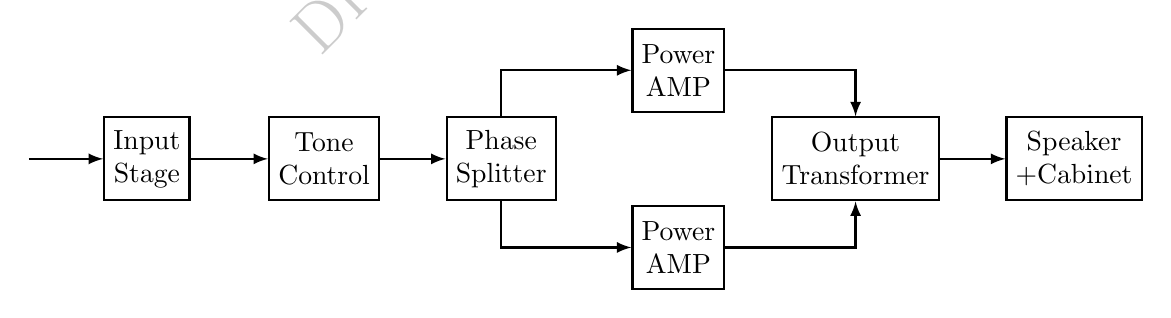
\begin{tikzpicture}[auto, thick, node distance=0.6cm, >=latex, scale = 0.75]
	\draw
	
	node at (0,0) [delay,align=center](d1) {Input\\Stage}
	node at (3,0) [delay,align=center] (d2){Tone\\Control}
	node at (6,0) [delay,align=center] (d3){Phase\\Splitter}
	node at (9,1.5) [delay,align=center] (d4){Power\\AMP}
	node at (9,-1.5) [delay,align=center] (d5){Power\\AMP}
	node at (12,0) [delay,align=center] (d6){Output\\Transformer}
	node at (15.7,0) [delay,align=center](d7){Speaker\\+Cabinet};

	
	\draw[->](-2,0)--(d1);
	\draw[->](d1)--(d2);
	\draw[->](d2)--(d3);
	\draw[->](d3)|-(d4);
	\draw[->](d3)|-(d5);
	\draw[->](d4)-|(d6);
	\draw[->](d5)-|(d6);
	\draw[->](d6)--(d7);
	\end{tikzpicture}
\end{center}
The main stages of a valve amplifier are given below:
\begin{itemize}
\item The $input\ stage$ consists of a triode circuit providing the input matching and preamplification followed by a volume control for the next stages.
\item  The $tone\ control$ circuitry is based on passive filter networks, typically with three controls for bass, mid and treble.
\item  The $phase\ splitter$ stage provides symmetrical power amp feeding. This phase splitter delivers the original input for the upper power amp and a phase inverted replica of the input for the lower power amp.
\item The $power\ amp$ stage in push-pull configuration performs individual amplification of the original and the phase inverted replica in a class A, class B or class AB configuration. The working point for class AB operation lies in-between class A and class B, also amplifying a part of the negative half wave. Class A and class AB are the main configurations for guitar power amplifiers.
\item  The $output\ transformer$ performs the subtraction of both waveforms delivered by the power amplifiers, which leads to a doubling of the output amplitude. The nonlinear behavior of transformers is beyond the scope of this discussion
\end{itemize}

\subsection{Speaker and cabinet} Guitar amplifiers are built either as a combo, where amplifier chassis and one or more loudspeakers are combined in the same enclosure or as a stack with separated amplifier head and loudspeaker cabinet. The traditional guitar cabinet is closed-back and houses four $12^{\prime \prime}$ speakers (4×12), but different combinations with loudspeakers in the range from $8^{\prime \prime}$ to $15^{\prime \prime}$ in closed or open enclosures are also available. The frequency responses of common guitar cabinets show an uneven bandpass characteristic with many resonances at mid frequencies. Simulations can be done by impulse response measurements of the loudspeaker and cabinet combination.

As well as the discussed topics, the influence of the power supply with valve rectifier is claimed to be of importance. A soft reduction of the power supply voltage occurs when in a high-power operation short transients need a high current. This power supply effect leads to a soft clipping of the audio signal. A proposal for tube simulation by using asymmetrical clipping is given by
\[
f(x)=\left\{\begin{array}{ll}{\frac{x-Q}{1-e^{-d i s t \cdot(x-Q)}}+\frac{Q}{1-e^{d i s t \cdot Q}},} & {Q \neq 0, x \neq Q,} \\ {\frac{1}{d i s t}+\frac{Q}{1-e^{d i s t} \cdot Q},} & {x=Q}\end{array}\right.
\]
The underlying design parameters for the simulation of tube distortion are based on the mathematical model where no distortion should occur when the input level is low (the derivative of $f(x)$ has to be $f^{\prime}(0) \approx 1$ and $f(0)=0$). The static characteristic curve should perform clipping and limiting of large negative input values and be approximately linear for positive values. 

The following {\bfseries Matlab} code performs the above function. To remove the dc component and to shape higher harmonics, additional lowpass and highpass filtering of the output signal is performed.
\begin{lstlisting}
function y = tube(audio, gain, Q, dist, rh, rl, mix)
% "Tube distortion" simulation, asymmetrical function
% x    - input
% gain - the amount of distortion, >0->
% Q    - work point. Controls the linearity of the transfer
%	     function for low input levels, more negative is more linear
% dist - controls the distortion's character, a higher number gives 
%	     a harder distortion, >0
% rh   - abs(rh)<1, but close to 1. Placement of poles in the HP 
%	     filter which removes the DC component
% rl   - 0<rl<1. The pole placement in the LP filter used to 
%	     simulate capacitances in a tube amplifier
% mix  - mix of original and distorted sound, 1=only distorted

q = audio * gain / max(abs(audio));			% Normalization
if Q == 0
	z = q ./ (1-exp(-dist*q));
	for i = 1: length(q)			% Test because of the
		if q(i) == Q				% transfer function's
			z(i) = 1 / dist;			% 0/0 value in Q
		end
	end
else
	z = (q-Q) ./ (1-exp(-dist*(q-Q))) + Q / (1-exp(dist*Q));
	for i = 1: length(q)				% Test because of the
		if q(i) == Q					% transfer function's
			z(i) = 1 / dist + Q / (1-exp(dist*Q));	% 0/0 value in Q
		end
	end
end
y = mix * z * max(abs(x)) / max(abs(z)) + (1-mix)*x;
y = y * max(abs(x)) / max(abs(y));			
y = filter([1 -2 1], [1 -2*rh rh^2], y);	% HP filter
y = filter([1-rl], [1 -rl], y);			    % LP filter

\end{lstlisting}
\section{Circuit-Based Valve Emulation}
Digital emulation of valve- or vacuum-tube amplifiers is currently a vibrant area of research with many commercial applications. As explained in a recent review article, most existing digital valve-emulation methods may roughly be divided into static waveshapers, custom nonlinear filters, and circuit-simulation-based techniques. The first type of these methods, static waveshapers use memoryless nonlinear functions for creating signal distortion and linear filtering before and after the nonlinearity for tuning the magnitude response. Oversampling is usually used to avoid signal aliasing.
\subsection{Dynamic Nonlinearities and Impedance Coupling}
Although the valve component itself is mainly a memoryless device that can in principle be approximated with static nonlinear functions, reactive components (typically capacitors) in the circuit make the nonlinearity act as dynamic. This means that in reality, the shape of the nonlinearity changes according to the input signal and the internal state of the circuit. Custom nonlinear valve emulation filters simulate this dynamic nonlinearity, for example by creating a feedback loop around the nonlinearity.

Another important phenomenon in real valve circuits is the two-directional impedance coupling between components and different parts of the circuit. This causes, for example, an additional signal-dependent bias variation of a valve circuit when connected to a reactive load, such as a loudspeaker. If the digital valve circuit model uses a unidirectional signal path – as many simple models do – altering some part in the virtual circuit has no effect on the parts earlier in the signal chain. For example, if a linear loudspeaker model is attached to a virtual tube circuit with unidirectional signal flow, the resulting effect will only be a linear filtering according to the transfer characteristics of the loudspeaker, and no coupling effects with the tube circuit will be present. Nonlinear circuit-simulation-based modeling techniques try to incorporate the impedance coupling effect, at least between some parts of the circuit. Traditionally, these methods use Kirchhoff’s rules and energy conservation laws to manually obtain the ordinary differential equations (ODEs) that represent the operation of the circuit. The ODEs are then discretized (usually using the bilinear transform), and the system of implicit nonlinear equations is iteratively solved using numerical integration methods, such as the Newton – Raphson or Runge – Kutta.
\subsection{Modularity}
From the digital valve-amplifier designer’s point of view, modularity would be a desirable property for the emulator. In an ideal system, it should be easy to edit the circuit topology, for example by graphically altering the circuit schematics, and the sonic results should be immediately available. Enabling full control over the digital circuit construction would allow the emulation of any vintage valve amplifier simply by copying its circuit schematics into the system. Furthermore, it would enable the designer to apply the knowledge of valve-amplifier building tradition into the novel digital models. Note that this would mean that the designer should not be limited by conventional circuit design constraints or even general physical laws in creating a new digital amplifier, so that also purely digital or “abstract” processing techniques could well be used in conjunction. In the late 1990s, several valve circuit models were presented for the SPICE circuit simulator software. Although these models were modular and able to simulate the full impedance coupling within the whole system, they could not be used as real-time effects due to their intensive computational load. In fact, even over a decade later, these SPICE models are computationally still too heavy to run in real time.

Wave digital filters (WDFs), introduced by Fettweis, offer a modular and relatively light approach for real-time circuit simulation. The main difference between WDFs and most other modeling methods is that WDFs represent all signals and states as wave variables and use local discretization for the circuit components. The WDF method will be explained more thoroughly in Section 3.3, and a simple nonlinear circuit simulation example using WDFs is presented in Section 3.4. The K-method, a state-space approach for the simulation of nonlinear systems has been introduced by Borin and others. This alternative approach for circuit simulation is currently another promising candidate for real-time valve simulation. It should be noted that although state-space models are not inherently modular, a novel technique by Yeh allows the automatization of the model-building process, so that state-space simulation models may automatically be obtained from a circuit schematics description.
\subsection{Wave Digital Filter Basics}
The basics of WDF modeling are briefly reviewed in the following section. A signal-processing approach has been chosen with less emphasis on the physical modeling aspects, in order to clarify the operation of the modeling example in Section 3.4
\subsubsection{One-Port Elements}

WDF components connect to each other using ports. Each port has two terminals, one for transport- ing incoming waves, and one for transporting outgoing waves. Also, each port has an additional parameter, port resistance, which is used in implementing proper impedance coupling between components. The relationship between the Kirchhoff pair (e.g., voltage U and current I) and wave variables A and B is given by
\[
\left[ \begin{array}{l}{A} \\ {B}\end{array}\right]=\left[ \begin{array}{c}{1+R_{\mathrm{p}}} \\ {1-R_{\mathrm{p}}}\end{array}\right] \left[ \begin{array}{c}{U} \\ {I}\end{array}\right] \Leftrightarrow \left[ \begin{array}{c}{U} \\ {I}\end{array}\right]=\frac{1}{2} \left[ \begin{array}{cc}{1} & {1} \\ {1 / R_{\mathrm{p}}} & {-1 / R_{\mathrm{p}}}\end{array}\right] \left[ \begin{array}{c}{A} \\ {B}\end{array}\right],
\]
where $R_{\mathrm{p}}$ denotes the port resistance.

Note that this port resistance is purely a computational parameter, and it should not be confused
with electrical resistance. Most elementary circuit components can be represented using WDF one-port elements. The port resistances of the one-port elements can be given as follows:
\[
R_{\mathrm{p}}=\left\{\begin{array}{ll}{R} & {\text { for resistance,}} \\ {1 /\left(2 C F_{\mathrm{s}}\right)} & {\text { for capacitance, }} \\ {2 L F_{\mathrm{s}}} & {\text { for inductance, }}\end{array}\right.
\]
where $R$, $C$ and $L$ are the electrical resistance (Ohms), capacitance (Farads), and inductance (Henrys), respectively, while $F_S$ stands for the sample rate (Hertz). Similar to the WDF resistor, the port resistance of a voltage source is equivalent to the physical resistance.
\subsubsection{Adaptors}
The WDF circuit components connect to each other via adaptors. In practice, the adaptors direct signal routing inside the WDF circuit model, and implement the correct impedance coupling via port resistances. Although the number of ports in an adaptor is not limited in principle, three-port adaptors are typically used, since any $N$-port adaptor ($N > 3$) can be expressed using a connection of three-port adaptors, so that the whole WDF circuit becomes a binary tree structure. There are two types of WDF adaptors: series and parallel, which implement the series and parallel connection between elements, respectively. Furthermore, the port resistance values for the adaptors should be set equal to the port resistances of the elements they are connected to. The outgoing wave $B_n$ at port $n = 1, 2, 3$ of a three-port adaptor can generally be expressed as
\[
B_{n}=\left\{\begin{array}{ll}{A_{n}-2 R_{n}\left(A_{1}+A_{2}+A_{3}\right) /\left(R_{1}+R_{2}+R_{3}\right)} & {\text { for series adaptor, }} \\ {2\left(G_{1} A_{1}+G_{2} A_{2}+G_{3} A_{3}\right) /\left(G_{1}+G_{2}+G_{3}\right)-A_{n}} & {\text { for parallel adaptor, }}\end{array}\right.
\]
where $A_n$ denotes the incoming wave at port $n$ and $G_n=1/R_n$ is the inverse of the port resistance $R_n$.
\subsubsection{Computational Scheduling}

The adaptors act as nodal points connecting the one-port elements together. For this reason, the adaptors in a WDF binary tree are also called nodes, and the one-port elements are called the leaves of the binary tree. When deciding the order of computations, a single one-port element must be chosen as the root of the tree. The nonlinear resistor is chosen as the root. When this decision has been made, the WDF simulation starts by first evaluating all the waves propagating from the leaves towards the root. When the incoming wave arrives at the root element, the outgoing wave is computed, and the waves are propagated from the root towards the leaves, after which the process is repeated.

As can be seen in above equation, the wave leaving the WDF adaptor is given as a function of the incoming waves and port resistances. This poses a problem for the computation schedule discussed above, since in order for the adaptor to compute the waves towards the root, it would also have to know the wave coming from the root at the same time. Interestingly, the port resistances can be used as a remedy. By properly selecting the port resistance for the port facing the root, the wave traveling towards the root can be made independent from the wave traveling away from the root.

For example, if we name the port facing the root element as port number one, and set its port resistance as $R_1 = R_2 + R_3$ if it is a series adaptor (and the inverse port resistance $G_1 = G_2 + G_3$ if it is a parallel adaptor), above equation simplifies into
\[
B_{1}=\left\{\begin{array}{ll}{-A_{2}-A_{3}} & {\text { for series connection, }} \\ {G_{2} /\left(G_{2}+G_{3}\right) A_{2}+G_{3} /\left(G_{2}+G_{3}\right) A_{3}} & {\text { for parallel connection, }}\end{array}\right.
\]
for the wave components traveling towards the root. In our example, the port number one would be called adapted, or reflection free, since the outgoing wave does not depend on the incoming
(reflected) wave. Such adapted ports are typically denoted with a “T-shaped” ending for the out- wards terminal, all adapted ports point towards the root.

Since the root element is connected to an adapted port, and the port resistances between the adapted port and the root should be equal, an interesting paradox arises. On one hand, the shared port resistance value should be set as required by the adaptor (for example as the sum of the other port resistances on a series adaptor), but on the other hand, the port resistance should be set as dictated by the root element (for example as a resistance value in Ohms for a resistor). If a resistor is chosen as a root element, the solution is to define the outgoing wave B from the root as
\[
B=\frac{R-R_{\mathrm{p}}}{R+R_{\mathrm{p}}} A
\]
where R is the electrical resistance of the root, Rp is the port resistance set by the adapted port, and A is the wave going into the root element. Since the port resistance of the adapted port is indepen- dent of the electrical resistance of the root, the latter can freely be varied during simulation without encountering computability problems. Thus, if the circuit has a nonlinear one-port element, it should be chosen as the root for the WDF tree (since nonlinearity can be seen as parametric variation at a signal rate). For all other leaves, changing the port resistance during simulation is problematic since correct operation would require the port resistance changes to be propagated throughout the whole tree and iterated to correctly set the changed wave values. In practice, however, it is possible to vary the port resistances (i.e., component values) of the leaves without problems, provided that the parametric variation is slow compared to the sampling rate of the system.
\subsubsection{Nonlinearities and Model Initialization}
In a nonlinear resistor, the electrical resistance value depends nonlinearly on the voltage over the resistor, and a correct simulation of this implicit nonlinearity requires iterative techniques in general. Note the difference between the earlier discussed global iteration for setting the values of all port resistances, and the local iteration to set only the value of the nonlinear resistor: although the adapted ports remove the need for the former, one should still in principle perform the latter. Since run-time iteration is a computationally intensive operation, a typical practical simplification for avoiding local iteration is to insert an additional unit delay to the system, for example by using the voltage value at the previous time instant when calculating the resistance value. The error caused by this extra delay is usually negligible, provided that the shape of the nonlinearity is relatively smooth, as is the case with typical valve components. Further information on nonlinear WDFs can be found. Valve simulation using WDFs was first presented and refined models have been discussed.

Reactive WDF circuit components should be correctly initialized before the simulation starts. This means that the one-sample memory of inductors and capacitors should be set so that the voltages and currents comply with Kirchhoff’s laws. For reactive components that have nonzero initial energy (for example an initially charged capacitor), this can be tricky since the relationship between the stored energy and the wave value inside the memory is not straightforward. However, the correct initialization procedure can still be performed by using The ́venin or Norton equivalents. A practical alternative is to set the memory of reactive WDF components to zero, and let the simula- tion run for some “warm-up” time before inserting the actual input signal so that a steady operating point is reached and the reactances have been properly charged. In a sense, this is similar to letting a real electric circuit warm up and reach the correct operating point before feeding the input signal.
\subsubsection{Remaining Challenges in WDF Modeling}
Although WDFs have many desirable properties in circuit-simulation applications, there are also some open research problems related to them that limit their usability on a large scale. Probably the most severe limitation is that those circuit topologies that do not map onto binary trees are difficult to realize. Such topologies include bridge connections and loop-like structures. Modeling of bridge connections using WDFs is further discussed. Another limitation is that a WDF binary tree can generally have only a single nonlinear element. If multiple nonlinearities are to be simulated using WDFs, global iteration should be applied for the whole sub-tree connecting the nonlinearities to each other. Alternatively, unit delays can be inserted into the system to enable computability, but this may drastically affect the stability of the system in some cases.
\subsubsection{Diode Circuit Model Using Wave Digital Filters}
This section discusses a WDF representation of a simple valve diode circuit. The simulator algorithm is implemented using object-oriented programming for illustrating the inherent modularity of WDFs. The related code requires a basic understanding of object-oriented programming principles, and is mainly intended to show the possibilities of WDF modeling, rather than trying to provide a computationally efficient implementation. The class files are defined in the following {\bfseries Matlab} code. The presented WDF simulator consists of seven classes, three of which are abstract (i.e., they only serve as superclasses to real classes). It must be noted that all the presented classes are shown in a single M-file for compactness although in practice MATLAB requires each class to reside in an individual file. In other words, the classes should be split into seven different files in order for the model to run in MATLAB.

The first class defines the WDF superclass, which serves as a parent for the other six classes. The $WDF$ class itself is inherited from MATLAB’s $hgsetget-class$, which results in all WDF elements being handle-objects. This means that when object properties (such as wave variable values) are edited, MATLAB only modifies the property values, instead of creating entirely new objects. The $PortRes$ property defines the port resistance of a WDF object, and the $Voltage$ method gives the voltage over the element. The next class defines the $Adaptor$ class, which serves as a superclass for three-port series and parallel adaptors. Two properties, $KidLeft$ and $KidRight$, are defined, which serve as handles to the WDF objects connected to the adaptor.

The $ser$ class defines the WDF series adaptor. The waves traveling up (towards the root) and down (away from the root) are given as properties $WU$ and $WD$, respectively. The adaptor is realized so that the adapted port always points up, to enable the connection of a nonlinear element at the root. In addition to the class constructor, this class defines two methods, WaveUp and set.WD. Note that the parallel adaptor is similarly defined and can be found among the supplementary MATLAB-files on-line, although it is omitted here for brevity.

The $OnePort$ class serves as a superclass for all one-port WDF elements. It also defines the up- and down-going waves $WU$ and $WD$ and the $set.WD$-method. This method also updates the internal state, or memory, of a reactive WDF one-port. The last three classes in M-file 12.6 introduce the classes $R$, $C$, and $V$, which represent the WDF resistors, capacitors, and voltage sources, respectively. Note that the class L for implementing a WDF inductor may easily be edited from the $C$ class, although it is not printed here (but included in the associated on-line code).
\begin{lstlisting}
%----------------------WDF Class------------------------
classdef WDF < hgsetget % the WDF element superclass
	properties 
		PortRes % the WDF port resistance
	end
	methods
		function Volts = Voltage(obj)  % the voltage (V) over a WDF element
			Volts = (obj.WU+obj.WD)/2; % as defined in the WDF literature
		end
	end
end
%----------------------Adaptor Class------------------------
classdef Adaptor < WDF % the superclass for ser. and par. (3-port) adaptors
	properties
		KidLeft % a handle to the WDF element connected at the left port
		KidRight % a handle to the WDF element connected at the right port
	end
end
%----------------------Ser Class------------------------
classdef ser < Adaptor % the class for series 3-port adaptors
	properties
		WD % this is the down-going wave at the adapted port
		WU % this is the up-going wave at the adapted port
	end
	methods 
		function obj = ser(KidLeft,KidRight) % constructor function
			obj.KidLeft = KidLeft; % connect the left 'child'
			obj.KidRight = KidRight; % connect the right 'child'
			obj.PortRes = KidLeft.PortRes+KidRight.PortRes; % adapt. port
		end
		function WU = WaveUp(obj) % the up-going wave at the adapted port
			WU = -(WaveUp(obj.KidLeft)+WaveUp(obj.KidRight)); % wave up
			obj.WU = WU; 
		end
		function set.WD(obj,WaveFromParent) %  sets the down-going wave
			obj.WD = WaveFromParent; % set the down-going wave for the adaptor
			% set the waves to the 'children' according to the scattering rules
			set(obj.KidLeft,'WD',obj.KidLeft.WU-(obj.KidLeft.PortRes/...
			obj.PortRes)*(WaveFromParent+obj.KidLeft.WU+obj.KidRight.WU)); 
			set(obj.KidRight,'WD',obj.KidRight.WU-(obj.KidRight.PortRes/...
			obj.PortRes)*(WaveFromParent+obj.KidLeft.WU+obj.KidRight.WU));
		end
	end 
end
%----------------------OnePort Class------------------------
classdef OnePort < WDF % superclass for all WDF one-port elements
	properties
		WD % the incoming wave to the one-port element
		WU % the out-going wave from the one-port element
	end
	methods 
		function obj = set.WD(obj,val) % this function sets the out-going wave
			obj.WD = val;
			if or(strcmp(class(obj),'C'),strcmp(class(obj),'L')) % if react.
				obj.State = val; % update internal state
			end
		end
	end 
end
%----------------------R Class------------------------
classdef R < OnePort % a (linear) WDF resistor
	methods 
		function obj = R(PortRes) % constructor function
			obj.PortRes = PortRes; % port resistance (equal to el. res.)
		end
		function WU = WaveUp(obj) % get the up-going wave
			WU = 0; % always zero for a linear WDF resistor
			obj.WU = WU;
		end
	end 
end
%----------------------C Class------------------------
classdef C < OnePort
	properties
		State % this is the one-sample internal memory of the WDF capacitor
	end
	methods 
		function obj = C(PortRes) % constructor function
			obj.PortRes = PortRes; % set the port resistance
			obj.State = 0; % initialization of the internal memory
		end
		function WU = WaveUp(obj) % get the up-going wave
			WU = obj.State; % in practice, this implements the unit delay
			obj.WU = WU;
		end
	end 
end
%----------------------V Class------------------------
classdef V < OnePort % class for the WDF voltage source (and ser. res.)
	properties
		E % this is the source voltage
	end
	methods 
		function obj = V(E,PortRes) % constructor function
			obj.E = E; % set the source voltage
			obj.PortRes = PortRes; % set the port resistance
			obj.WD = 0; % initial value for the incoming wave
		end
		function WU = WaveUp(obj) % evaluate the outgoing wave
			WU = 2*obj.E-obj.WD; % from the def. of the WDF voltage source
			obj.WU = WU;
		end
	end 
end
\end{lstlisting}
The actual diode simulation example is printed as following {\bfseries Matlab} code, and will be briefly explained here. it tarts by defining the overall simulation parameters and variables, such as the sample rate, and input and output signals. Next, the WDF elements (resistive voltage source, resistor, and a capacitor) are created, and the WDF is formed as a series connection. The nonlinear resistor is not created as an object, but it is manually implemented in the simulation loop.

The simulation loop starts by reading the input signal as the source voltage for object V1. Next, the $WaveUp$ method is called for the WDF tree, resulting in all up-going waves to be propagated at the root. The valve resistor is modeled as the nonlinear resistance
\[
R=125.56e^{-0.036U}\Omega
\]
as a function of the voltage $U$ over the diode. Equation was empirically found to be a simple, but fairly accurate simulation of a GZ 34 valve diode. Here, the previous value of the diode voltage is used, in order to avoid the local iteration of the implicit nonlinearity. The wave reflection at the nonlinearity is implemented, and the down-going waves are propagated to the leaves. Finally, the diode voltage is updated for the next time sample, and the output is read as the voltage over the resistor $R1$. After the simulation loop is finished, the results are illustrated using the plot-commands.

It is important to note, that due to the modularity of the WDFs and the object-oriented nature of the implementation, editing of the simulation circuit is very easy. All that has to be done to simulate a different circuit is to change the one-port element definitions. In other words, the two M-files define an entire circuit simulation software!
\begin{lstlisting}
Fs = 20000; % sample rate (Hz)
N = Fs/10; % number of samples to simulate
gain = 30; % input signal gain parameter
f0 = 100; % excitation frequency (Hz)
t = 0:N-1; % time vector for the excitation
input = gain.*sin(2*pi*f0/Fs.*t); % the excitation signal
output = zeros(1,length(input));
V1 = V(0,1); % create a source with 0 (initial) voltage and 1 Ohm ser. res.
R1 = R(80); % create an 80Ohm resistor
CapVal = 3.5e-5; % the capacitance value in Farads
C1 = C(1/(2*CapVal*Fs)); % create the capacitance
s1 =  ser(V1,ser(C1,R1)); % create WDF tree as a ser. conn. of V1,C1, and R1
Vdiode = 0; % initial value for the voltage over the diode
%% The simulation loop:
for n = 1:N % run each time sample until N
	V1.E = input(n); % read the input signal for the voltage source
	WaveUp(s1); % get the waves up to the root
	Rdiode = 125.56*exp(-0.036*Vdiode); % the nonlinear resist. of the diode
	r = (Rdiode-s1.PortRes)/(Rdiode+s1.PortRes); % update scattering coeff.
	s1.WD = r*s1.WU; % evaluate the wave leaving the diode (root element)
	Vdiode = (s1.WD+s1.WU)/2; % update the diode voltage for next time sample
	output(n) = Voltage(R1); % the output is the voltage over the resistor R1
end 
%% Plot the results
t = (1:length(input))./Fs; % create a time vector for the figure
hi = plot(t,input,'--'); hold on; % plot the input signal, keep figure open
ho = plot(t,output); hold off; % plot output signal, prevent further plots
grid on; % use the grid for clarity
xlabel('Time (s)'); ylabel('Voltage (V)'); % insert x- and y-axis labels
legend([hi ho],'Source voltage E','Voltage over R1'); % insert legend

\end{lstlisting}
\end{document}
